\documentclass[10pt,twocolumn,letterpaper]{article}

\usepackage{cvpr}
\usepackage{times}
\usepackage{epsfig}
\usepackage{graphicx}
\usepackage{amsmath}
\usepackage{amssymb}

% Include other packages here, before hyperref.
\usepackage{lipsum}
\usepackage{subcaption}
\usepackage{url}

\usepackage[breaklinks=true,bookmarks=false]{hyperref}

\cvprfinalcopy 

\def\cvprPaperID{****}
\def\httilde{\mbox{\tt\raisebox{-.5ex}{\symbol{126}}}}

\setcounter{page}{1}
\begin{document}

%%%%%%%%% TITLE
\title{Project for Gallerie Estensi Museum\\
\large Group n. 26}

\author{
Luca Denti\\
{\tt\small 211805@studenti.unimore.it}
\and
Cristian Mercadante\\
{\tt\small 213808@studenti.unimore.it}
\and
Alberto Vitto\\
{\tt\small 214372@studenti.unimore.it}
}

\maketitle

%%%%%%%%% ABSTRACT
\begin{abstract}
We propose an approach to detect, retrieve and rectify paintings in videos shot in Gallerie Estensi museum located in Modena as project of the \emph{Vision and Cognitive Systems} master's degree course. We applied image processing algorithms such as adaptive thresholding, morphology operators and obtained the contours of the paintings. Through SIFT keypoints we found the ranking of the matches with the paintings in the database and used the best one to find a perspective transformation that could correct the detection. With a YOLO pretrained network we identified the people and then, based on the outcome of the retrieval, we located the room of the museum. Our pipeline showed good results in detection, even without applying learning techniques. The retrieval system also proved to be satisfactory, as well as YOLO.
\end{abstract}

%%%%%%%%% BODY TEXT

\section{Introduction}
\label{sec:Introduction}
The purpose of this report is to show a possible application of Computer Vision in the cultural and tourism sector, using visual data coming from Gallerie Estensi of Modena. This project started as a group activity for the \textit{Vision and Cognitive Systems} course of the master's degree in Computer Engineering of the University of Modena and Reggio Emilia. Professors Rita Cucchiara and Lorenzo Baraldi provided the material, knowledge and support for carrying out the activity, indicating the tasks and milestones to be achieved:
\begin{itemize}
    %\setlength\itemsep{-0.5em}
    \item Painting detection: given a video, detect paintings in each frame;
    \item Painting retrieval: match each detected painting to the corresponding original image in the dataset;
    \item Painting rectification: correct the perspective distortion of each detected painting;
    \item People detection: detect each person in every frame of the given video;
    \item People localization: localize every person detected.
\end{itemize}

\subsection{Dataset}
\label{subsec:Dataset}
The dataset we worked on consists of 208 videos acquired from various cameras, in particular GoPro and smartphones, 95 unique images for each painting in the gallery (actually this images dataset was not complete with all the paintings present in Gallerie Estensi), a spreadsheet with information on paintings and a map of the gallery. The videos have some features that required special attention:
\begin{itemize}
    \item illumination not always optimal for the identification of the paintings;
    \item overlapping of people and paintings;
    \item highly distorted paintings that appear as one due to perspective;
    \item rapid movement of the camera causing blurred frames.
\end{itemize}

We have also manually labeled 285 frames, sampled every second from 14 randomly selected videos in the dataset, in order to use them as a test set for painting detection and retrieval tasks and compute some performance measures.

\subsection{Overview}
\label{subsec:Overview}
We now present an overview of what will follow:
\begin{itemize}
    \item Chapter \ref{sec:PaintingDetection} describes the preprocess pipeline and the subsequent identification of the regions of interest, using denoising and morphological functions from OpenCV.
    \item Chapter \ref{sec:PaintingRetrieval} describes the usage of SIFT \cite{10.1023/B:VISI.0000029664.99615.94} to retrieve the original images from the dataset, according to the detections.
    \item Chapter \ref{sec:PaintingRectification} describes the usage of SIFT to rectify the detected images, according to descriptor matches.
    \item Chapter \ref{sec:PeopleDetectionAndLocalization} describes the application of the YOLO \cite{redmon2015unified} network and our approach on localizing each person in the room.
    \item Chapter \ref{sec:ResultsAndConclusion} is dedicated to various evaluation tests with precision, recall, accuracy, mAP measures and a conclusion with future improvements.
\end{itemize}

\section{Painting detection}
\label{sec:PaintingDetection}
The goal of painting detection is to predict a ROI (region of interest), \ie a bounding box around each painting.
To deal with this task, our approach was to find a candidate contours set that could contain most of the paintings (ideally, 0 false negatives and a lot of false positives), and then make some refinements to discard contours that don't correspond to a painting (ideally, 0 false negatives and 0 false positives).
Therefore, the detection involves two main steps:
\begin{itemize}
\item creation of the candidate contours set
\item discarding of the \textit{not-painting} contours
\end{itemize}

First of all, we apply some processing functions to obtain a binary image on which the candidate painting contours could be better found (as shown in figure \ref{fig:PaintingDetectionPipeline}):
\begin{enumerate}
    \item adjust brightness and contrast
    \item convert to gray-scale
    \item apply a bilateral filter
    \item apply adaptive threshold
    \item apply morphology methods (closing)
\end{enumerate}

Secondly, we apply the OpenCV function \texttt{findContours} \cite{journals/cvgip/SuzukiA85}, which implements a border following algorithm to retrieve the contours from a binary image, and build our candidate set.
For each candidate contour, we obtain the convex hull, the contour approximation with \texttt{approxPolyDP} \cite{approxPolyDP} (Ramer–Douglas–Peucker algorithm), the minimum area (rotated) bounding rectangle, the ellipse inscribed in the rotated rectangle and the bounding box itself. All of these are required for computing some checks, and if at least one of them is not verified, than the corresponding contour will be discarded:
\begin{enumerate}
    \item Minimum number of points of convex hull and \texttt{approxPolyDP}: if it's lower than a threshold (\eg 4) we suppose no painting is found;
    \item Maximum aspect ratio of the bounding box: we suppose paintings have a maximum aspect ratio (width/height and vice versa); 
    \item Minimum variance of the color histogram: if it's lower than a threshold, we suppose that no painting is found because the region is somehow too flat in terms of color;
    \item Maximum value of the 80-percentile of the grayscale histogram: we suppose that areas with too much brightness must be discarded;
    \item Minimum rotated/elliptical bounding box area percentage with respect to the convex hull area: the idea is that a rectangular/elliptical painting should have a convex hull that covers most of the rotated/elliptical bounding box area;
    \item Minimum \texttt{approxPolyDP} area percentage with respect to the convex hull area: the same concept as in the previous point;
    \item Minimum convex hull area percentage with respect to the image area: we discard contours that are too small compared to the whole image;
    \item Minimum convex hull area percentage with respect to the widest convex hull found: we discard contours that are too small compared to the widest painting found.
\end{enumerate}

In section \ref{subsec:PaintingDetectionEvaluation} we will show the results of this approach on the test set mentioned in section \ref{subsec:Dataset}.

\begin{figure}[t]
\begin{center}
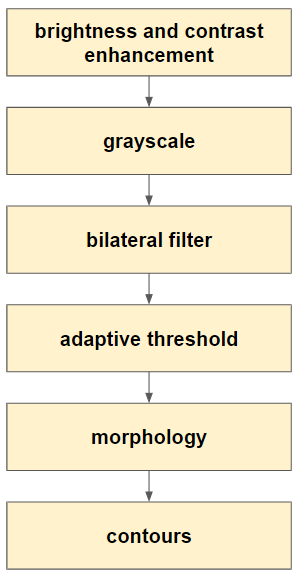
\includegraphics[width=0.5\linewidth]{images/image5.png}
\end{center}
\caption{Image processing pipeline for painting detection.}
\label{fig:PaintingDetectionPipeline}
\end{figure}

\begin{figure*}[]
  \centering
  \begin{tabular}{cc}
    \subcaptionbox{Brightness, contrast enhancement and smoothing.\label{fig:PaintingDetectionSmoothing}}[0.45\linewidth]{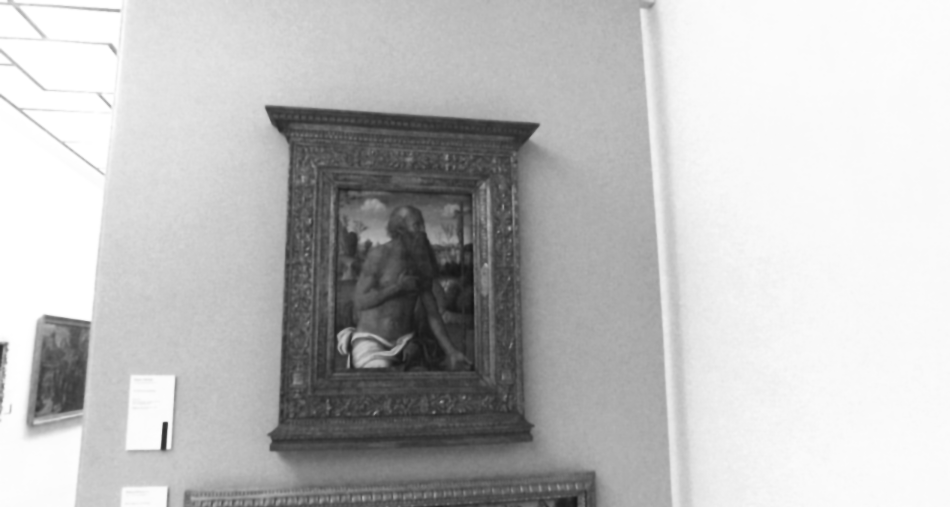
\includegraphics[width=\linewidth]{images/image8.png}} &
    \subcaptionbox{Adaptive thresholding.\label{fig:PaintingDetectionThresholding}}[0.45\linewidth]{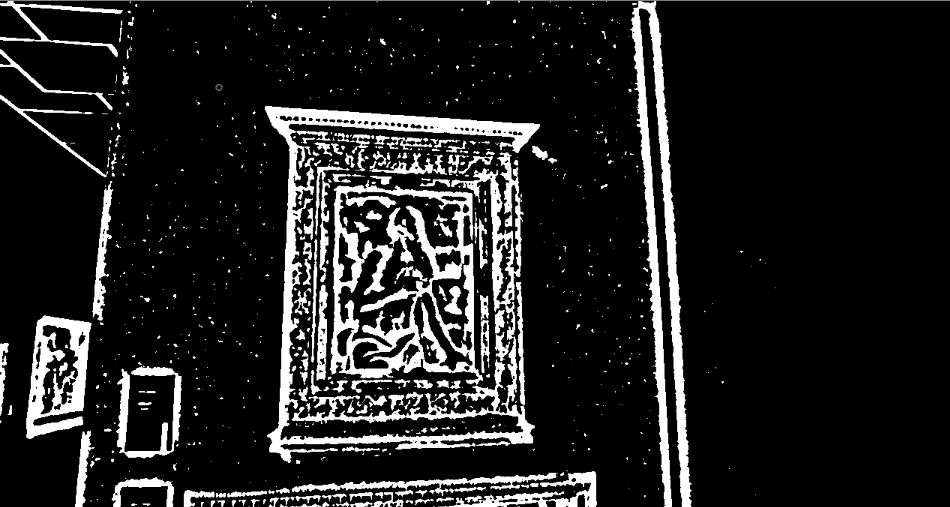
\includegraphics[width=\linewidth]{images/image6.png}} \\
    \subcaptionbox{Closing operator.\label{fig:PaintingDetectionClosing}}[0.45\linewidth]{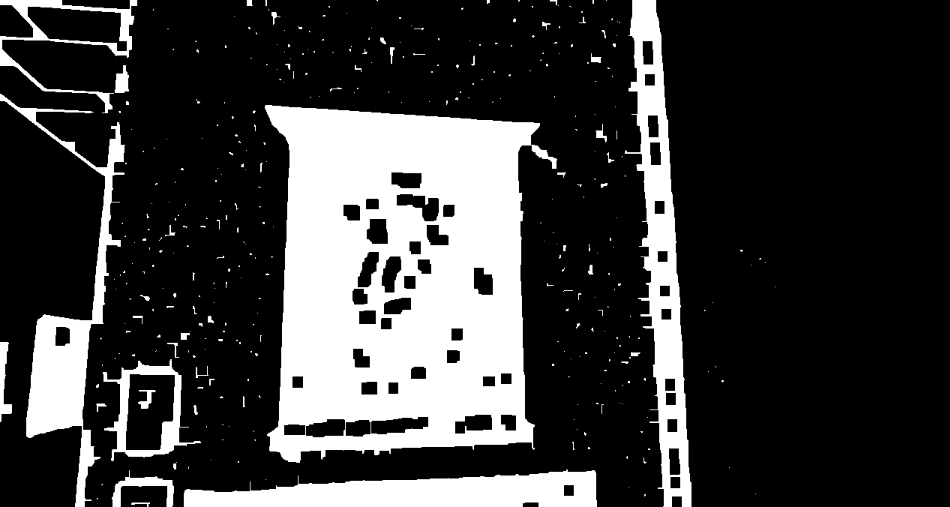
\includegraphics[width=\linewidth]{images/image9.png}} &
    \subcaptionbox{Result.\label{fig:PaintingDetectionResult}}[0.45\linewidth]{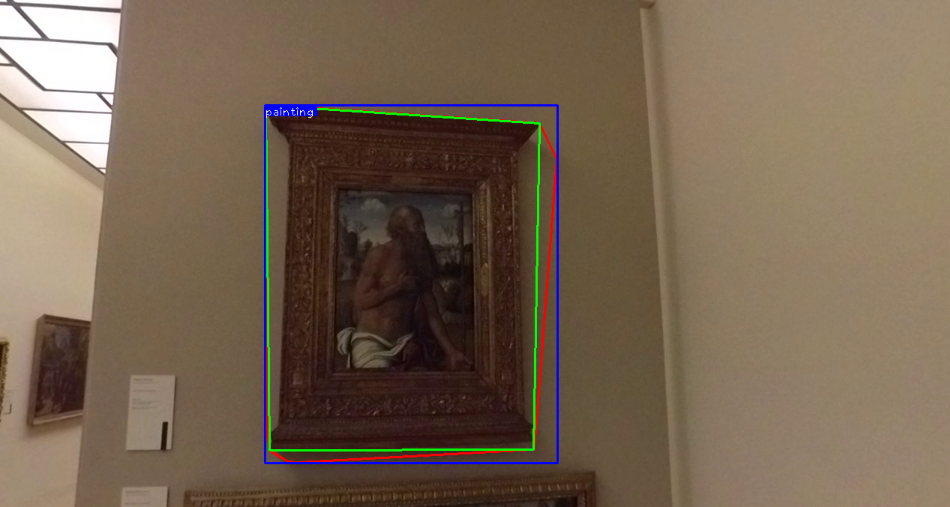
\includegraphics[width=\linewidth]{images/image4.png}}
  \end{tabular}
  \caption{Visualization of the preprocessing pipeline for painting detection.\label{fig:PaintingDetectionImages}}
\end{figure*}


\section{Painting retrieval}
\label{sec:PaintingRetrieval}
Given a painting ROI, the goal of painting retrieval is to obtain a ranked list of all the paintings in the database, sorted by descending order of similarity with respect to the input. Ideally, the first element of that list should be the corresponding real painting.

First of all, we extracted SIFT \cite{10.1023/B:VISI.0000029664.99615.94} keypoint descriptors for every image in the database and created two lists: one with the descriptors and the other with the indices of the database paintings where the descriptors were taken from. Finally, we stored these lists in two files, called respectively \texttt{features\textunderscore db.npy} and \texttt{img\textunderscore features\textunderscore db.npy}.
These two lists are used to train a kNN classifier: the first one contains the training instances and the second contains their classes.
When a new painting ROI is passed to the system, we extract its SIFT keypoint descriptors. We create a frequency vector of length equal to the number of classes (\ie 95).
For each descriptor, we ask the classifier to predict the nearest neighbor class (\ie it finds the most similar training descriptor and returns its class) and we increment the corresponding counter in the frequency vector. We obtain the ranked list by sorting the vector in descending order.

The main problem with this approach is that if we take the ROI image as it is, performance is quite low. The reason is that the ROI always includes the frame and many SIFT keypoints are found in it. Since the majority of the images in the database don't have the frame, those SIFT keypoints will match with random keypoints and thus the ranking list will be wrongly built.
To solve this problem, we apply an elliptical mask over the ROI image. In this way, we keep only the central part of the image, possibly discarding the frame. There are some assumptions for this method to work:
\begin{itemize}
    \item The ROI must have the painting as central as possible;
    \item In case of rectangular paintings, the elliptical mask will discard not only the frame but also the four parts at the corners. This can be acceptable because typically the subjects are centered in the paintings and consequently also the majority of the details (\ie keypoints).
\end{itemize}

Since many paintings are missing from the database, we also took into account the situation where input can't be matched with any real painting. In this case, the first element of the ranking will be wrong. Our approach was to identify this situation and automatically insert in the first position of the ranking list the value -1. 
After creating the ranking list, our system can make an extra check on the first element to make sure it's likely to match. We extract the SIFT keypoint descriptors of the first rank image from the database and the ones from the input image. We use \textit{Fast Library for Approximate Nearest Neighbors} (FLANN) \cite{Muja09fastapproximate} implemented in OpenCV as a matcher between the SIFT descriptors, then apply the Lowe's ratio test to leave out less reliable matches. If the number of matches is lower than a threshold (\eg 10), then we can state that the input and the predicted painting actually don't match and we can insert the value -1 in the ranking.

In section \ref{subsec:PaintingRetrievalEvaluation}, we will show the results of this approach on the test set mentioned in section \ref{subsec:Dataset}.

\section{Painting rectification}
\label{sec:PaintingRectification}
By rectification we mean the application of a perspective transformation of a painting detection such as to show the painting in its entirety from a frontal point of view. To solve this task in the best way, it would have been necessary to have the parameters of the cameras used to record the videos of the dataset, in order to extrapolate the real dimensions of the identified paintings, correct the distortion and be able to reconstruct the image from the rectified painting. However, the parameters of the cameras were not included in the dataset, therefore it is difficult to reconstruct the aspect ratio of the original painting. Furthermore, the distortion correction would never have been uniform for all the videos in the dataset, given that they come from different sources and that in production stage there may be an unknown camera. Therefore we have decided to ignore the problem, since the method we are going to illustrate works very well even with distorted images.
Hence, we have chosen to rectify the detected painting only after recovering the corresponding original painting from the images dataset: in this way we have the original proportions of the painting so we can apply a perspective transformation. To obtain the transformation matrix, we calculated two feature vectors using SIFT: one over the recovered painting, the other over the detected painting from the video and we used \textit{Fast Library for Approximate Nearest Neighbors} (FLANN) implemented in OpenCV as a matcher between the SIFT descriptors, then apply the Lowe's ratio test to leave out less reliable matches. Next we extracted the coordinates of the key points both in the detection and in the original image and applied RANSAC \cite{10.1145/358669.358692} to obtain the projection matrix. In this way the outputs are not only corrected, but also proportionate and exclude the frame of a painting if the image in the dataset doesn't have it.

Our approach is very effective, but it assumes that the retrieval is correct: however, often it fails due to the lack of the corresponding images in the dataset. For this reason in these cases we used a simpler approach that doesn’t keep proportions but tries to rectify.
We apply a preprocess pipeline similar to the one described in section \ref{sec:PaintingDetection} for painting detection on the ROI image. We find the contours and keep only the biggest one in terms of area. We assume that it corresponds to the painting contour. Then, we obtain the coordinates of the top-left, top-right, bottom-right and bottom-left points from the contour points list. 
We would like to project these points on the four corners of the warped image. To find the corners we need to determine the dimensions of the new image. We compute the width as the largest distance between the bottom-right and bottom-left x-coordinates or the top-right and top-left x-coordinates. Similarly, we compute the height as the maximum distance between the top-right and bottom-right y-coordinates or the top-left and bottom-left y-coordinates.  
We are now able to define the corners coordinates of the warped image: \texttt{(0, 0)} indicating the top-left corner, \texttt{(width-1, 0)} which is the top-right, \texttt{(width-1, height-1)} which is the bottom-right and \texttt{(0, height-1)} is the bottom-left.
From these four pair of coordinates we can retrieve the homography transformation matrix which is applied to the ROI image. The output is the rectified painting image.
This method works obviously better on rectangular paintings, since for elliptical paintings we can't determine if they are actually elliptical paintings or just circular but in perspective.

\begin{figure}[t]
\begin{subfigure}[b]{\linewidth}
    \begin{center}
    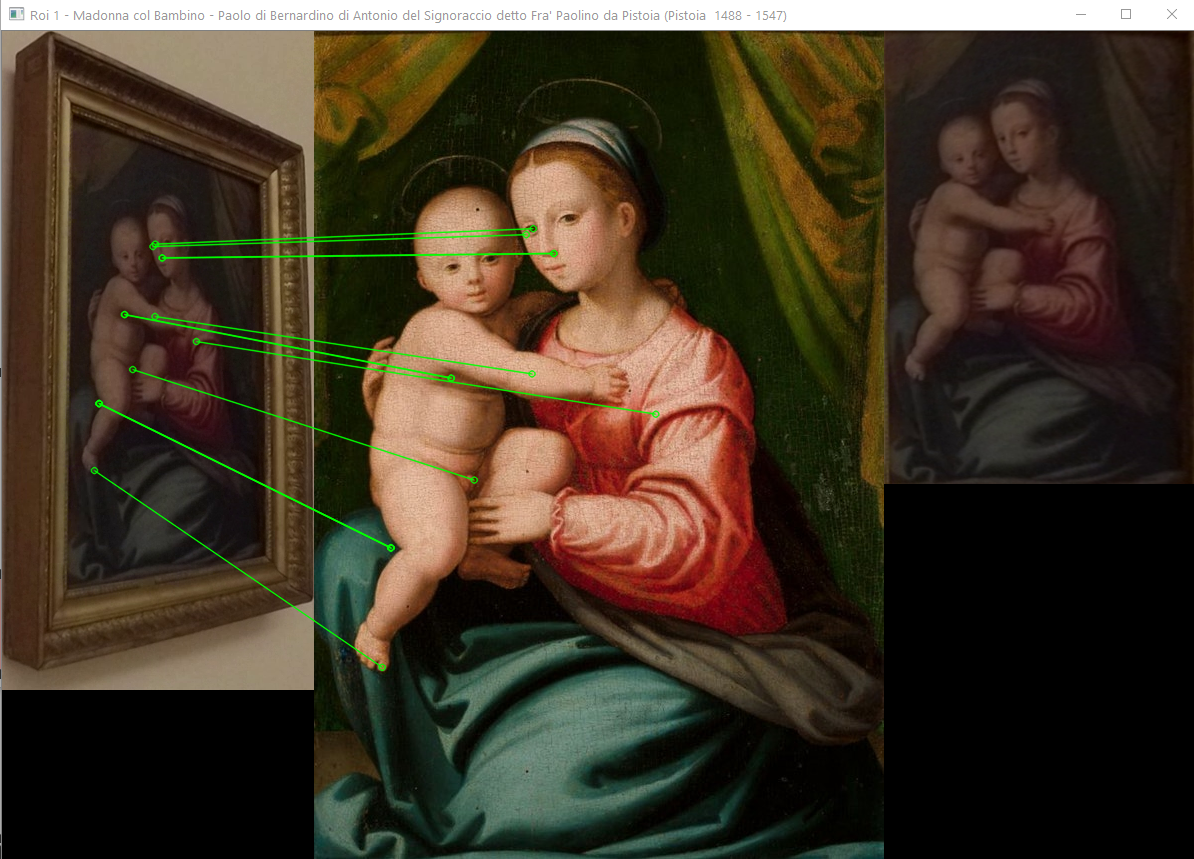
\includegraphics[width=\linewidth]{images/image10.png}
    \end{center}
    \caption{Result obtained applying a perspective transformation using SIFT matches.}
    \label{fig:PaintingRectificationSIFT}
\end{subfigure}
\begin{subfigure}[b]{\linewidth}
%    \hspace{1.5cm}
    \begin{center}
    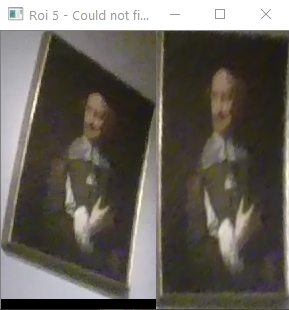
\includegraphics[width=0.6\linewidth]{images/image7.png}
    \end{center}
    \caption{Result obtained without SIFT matches.}
    \label{fig:PaintingRectificationNoSIFT}
\end{subfigure}
\caption{Visualization of the two approaches on painting rectification as described in section \ref{sec:PaintingRectification}.}
\label{fig:PaintingRectificationImages}
\end{figure}

\section{People detection and localization}
\label{sec:PeopleDetectionAndLocalization}

\begin{figure*}[t]
\begin{center}
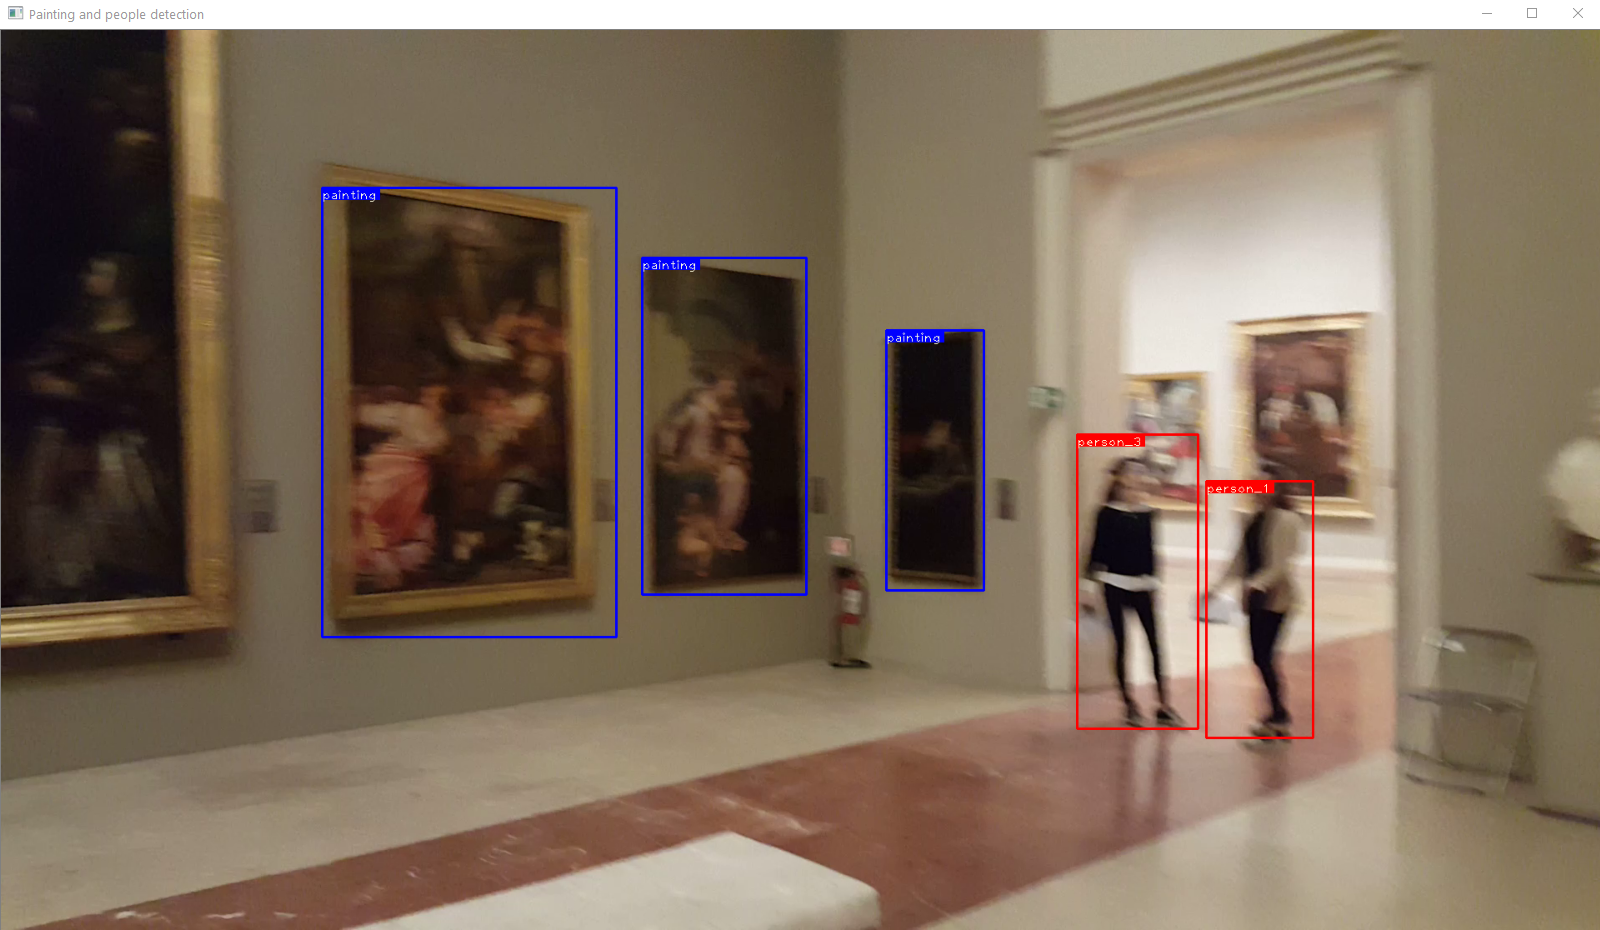
\includegraphics[width=0.8\linewidth]{images/image3.png}
\end{center}
\caption{Example of output with both paintings and people detection.}
\label{fig:PeopleDetection}
\end{figure*}

Some videos in the dataset also include visitors: our goal is to identify people and indicate which room in the museum they are in. We decided to use YOLO \cite{redmon2015unified}, a multi-class network for detection, one of which is people. It would have been difficult to identify people in the same way in which we identified the paintings (by applying classic image processing), as these have a typically known geometric shape, are static and always present only one point of view. Instead people could be framed in part, present themselves with different profiles, etc. Hence the choice to opt for a pre-trained neural network. The model we use is able to recognize up to 80 classes, but for our use we have taken into consideration only the detection of people.

The problem with this approach relates to the fact that the detection of paintings and people use different methodologies and do not communicate with each other: It may happen that the neural network identifies the people depicted in the paintings as real people, thus creating false positives. To overcome this problem we have added checks on the position of the person's ROI with respect to the ROIs of the panels: for each identified person we verify if the area of the person's ROI is totally included in the area of a painting's ROI and if true we discard the detection of the person.
\begin{equation}
\label{eq:DiscardPerson}
Area_{person} \cap Area_{painting} = Area_{person}
\end{equation}

This approach works in most cases, but is based on the assumption that the system correctly identifies the paintings: if one of those is not recognized, potentially the system will output the people depicted within it. Another problem is that YOLO sometimes recognizes statues as person. So, in order to have better results we applied a threshold to the confidence score on each person detection. Given that both statues and people depicted inside the paintings are very realistic, sometimes those detection have a confidence varying from 0.40 to 0.95. Instead, a real people detection usually has a score higher than 0.97, so we applied a threshold of 0.96. However, YOLO's confidence is still high when we have colored and realistic statues (as in figure \ref{fig:PeopleDetectionError})

\begin{figure}[t]
\begin{center}
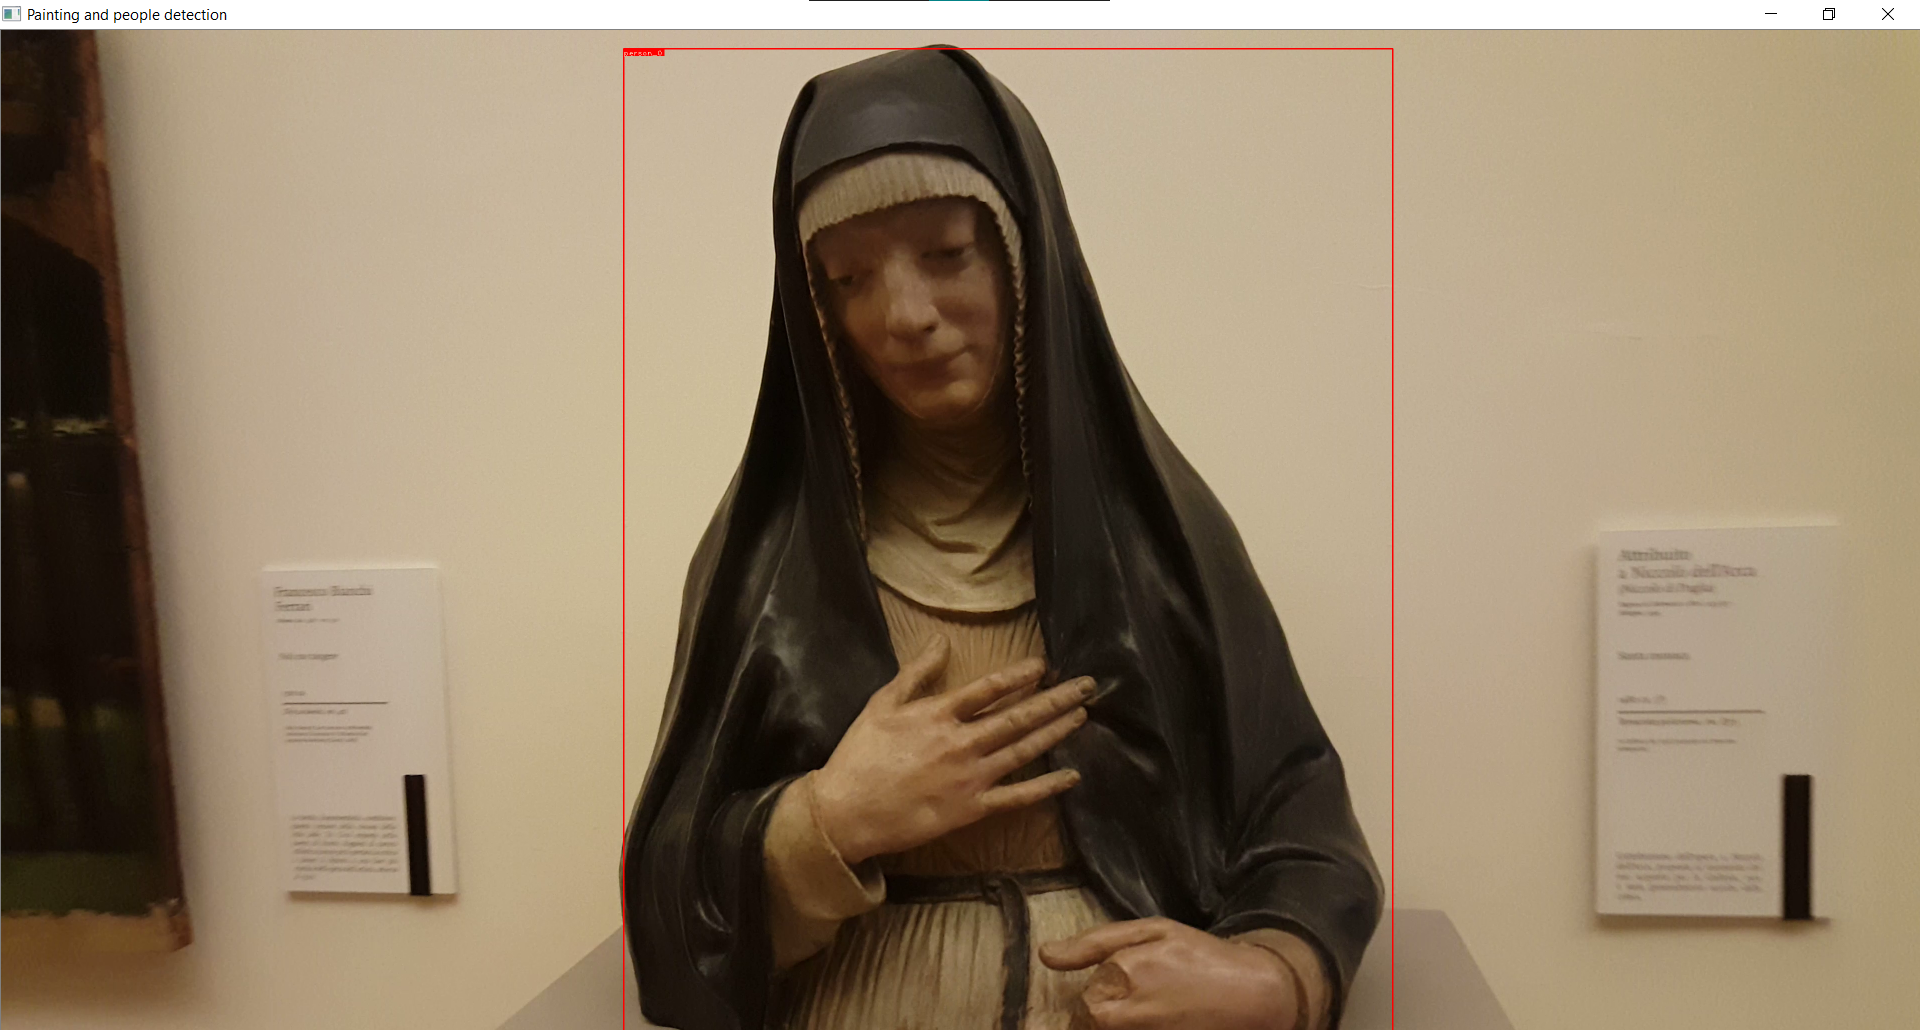
\includegraphics[width=\linewidth]{images/madonna.png}
\end{center}
\caption{Statue wrongly recognized as a person.}
\label{fig:PeopleDetectionError}
\end{figure}

The localization phase requires to indicate for each person present in the video the position inside the museum, that is the room. Since it is very rare that people are framed in rooms adjacent to the one in which the room is located, we have simplified the task: we simply show the room in which the camera is recording. To do this we need the retrieval of the detected paintings and then do a lookup on the \texttt{data.csv} file which contains information on the paintings, such as the author, the name and the room number. We therefore use the room number to show the current room. To deal with possible errors in the retrieval phase, we use a simple voting system on the number of rooms to be shown in the output. This consists of the \texttt{map.png} file, in which we insert a colored overlay in correspondence of the current room.

\section{Results and conclusion}
\label{sec:ResultsAndConclusion}
\subsection{Painting detection evaluation}
\label{subsec:PaintingDetectionEvaluation}

The evaluation phase was conducted on the test set mentioned in section \ref{subsec:Dataset}.
A predicted bounding box is considered correct (TP) if there is a ground-truth bounding box which is labelled with class \textit{painting} and the IoU (Intersection over Union) metric between the two boxes is above a threshold, typically 0.5.
For each video in the test set, we evaluated the frames, counted the number of TP, FP and FN and computed the average precision and recall. Finally, we obtained the precision and recall and the F1 score for the overall test set, as a mean of the average precision and recall of the single videos.
Table \ref{tab:PaintingDetectionResults1} presents the results we obtained with the whole painting detection pipeline (both the 2 steps) as introduced in section \ref{sec:PaintingDetection}. Instead, table \ref{tab:PaintingDetectionResults2} presents the results without the checks for \textit{not-painting} contours (only step 1). As we expected, the recall in table \ref{tab:PaintingDetectionResults2} is quite high and the precision is drastically low. Consequently, our system was able to improve the precision while not sacrificing too much the recall. 
However, there are some limitations in performance due to:
\begin{itemize}
    \item paintings seen only partially (either because occluded or zoomed in too much).
    \item paintings strongly in perspective (sometimes two paintings are incorporated into only one contour).
    \item paintings overlapped with other artifacts or people.
\end{itemize}

\begin{table}[]
\begin{center}
\begin{tabular}{lrrrrrrr}
\multicolumn{1}{c}{\textbf{Video}} & \multicolumn{1}{c}{\textbf{TP}} & \multicolumn{1}{c}{\textbf{FP}} & \multicolumn{1}{c}{\textbf{FN}} & \multicolumn{1}{c}{\textbf{TN}} & \multicolumn{1}{c}{\textbf{P}} & \multicolumn{1}{c}{\textbf{R}} & \multicolumn{1}{c}{\textbf{F1}} \\ \hline \hline
000 & 39 & 8 & 29 & 0 & 0.83 & 0.57 &  \\
001 & 73 & 5 & 26 & 0 & 0.94 & 0.74 &  \\
002 & 106 & 10 & 47 & 0 & 0.91 & 0.69 &  \\
003 & 85 & 4 & 67 & 0 & 0.96 & 0.56 &  \\
004 & 0 & 0 & 0 & 0 & 1 & 1 &  \\
005 & 11 & 1 & 6 & 0 & 0.92 & 0.65 &  \\
006 & 16 & 0 & 1 & 0 & 1 & 0.94 &  \\
007 & 6 & 0 & 3 & 0 & 1 & 0.67 &  \\
008 & 61 & 0 & 17 & 0 & 1 & 0.78 &  \\
009 & 45 & 7 & 27 & 0 & 0.87 & 0.62 &  \\
010 & 29 & 5 & 34 & 0 & 0.85 & 0.46 &  \\
012 & 16 & 0 & 4 & 0 & 1 & 0.8 &  \\
013 & 30 & 7 & 20 & 0 & 0.81 & 0.6 &  \\
014 & 76 & 6 & 16 & 0 & 0.93 & 0.83 &  \\ \hline \hline
\textbf{Total} &  &  &  &  & \textbf{0.93} &\textbf{ 0.71} & \textbf{0.8} \\
\end{tabular}
\end{center}
\caption{Painting detection results with checks for \textit{not-paintings}, where \textit{P} is precision and \textit{R} is recall}
\label{tab:PaintingDetectionResults1}
\end{table}

\begin{table}[]
\begin{center}
\begin{tabular}{lrrrrrrr}
\multicolumn{1}{c}{\textbf{Video}} & \multicolumn{1}{c}{\textbf{TP}} & \multicolumn{1}{c}{\textbf{FP}} & \multicolumn{1}{c}{\textbf{FN}} & \multicolumn{1}{c}{\textbf{TN}} & \multicolumn{1}{c}{\textbf{P}} & \multicolumn{1}{c}{\textbf{R}} & \multicolumn{1}{c}{\textbf{F1}} \\ \hline \hline
000 & 49 & 17587 & 19 & 0 & 0 & 0.72 &  \\
001 & 97 & 2849 & 2 & 0 & 0.03 & 0.98 &  \\
002 & 141 & 3850 & 12 & 0 & 0.04 & 0.92 &  \\
003 & 127 & 6636 & 25 & 0 & 0.02 & 0.84 &  \\
004 & 0 & 1738 & 0 & 0 & 0 & 1 &  \\
005 & 17 & 18195 & 0 & 0 & 0 & 1 &  \\
006 & 17 & 1320 & 0 & 0 & 0.01 & 1 &  \\
007 & 9 & 6466 & 0 & 0 & 0 & 1 &  \\
008 & 67 & 1039 & 11 & 0 & 0.06 & 0.86 &  \\
009 & 65 & 3071 & 7 & 0 & 0.02 & 0.9 &  \\
010 & 42 & 972 & 21 & 0 & 0.04 & 0.67 &  \\
012 & 20 & 4496 & 0 & 0 & 0 & 1 &  \\
013 & 49 & 2074 & 1 & 0 & 0.02 & 0.98 &  \\
014 & 92 & 632 & 0 & 0 & 0.13 & 1 &  \\ \hline \hline
\textbf{Total} &  &  &  &  & \textbf{0.03} & \textbf{0.92} & \textbf{0.05} \\
\end{tabular}
\end{center}
\caption{Painting detection results without checks for \textit{not-paintings}, where \textit{P} is precision and \textit{R} is recall}
\label{tab:PaintingDetectionResults2}
\end{table}

\subsection{Painting retrieval evaluation}
\label{subsec:PaintingRetrievalEvaluation}
Given the frames of a video in the test set, for each correctly detected ROI, we obtain the ranking list. According to the value of the corresponding ground truth label, we have three cases:
\begin{itemize}
    \item If the ground truth label is at position $p$ within the first \texttt{rank\_scope} (\eg 5) items of the list, then the precision for that detection will be $1/p$;
    \item If the ground truth label is not in the first \texttt{rank\_scope} positions of the list, then the precision for that detection will be 0;
    \item If the ground truth label is -1, then we skip this detection because the painting was not in the dataset.
\end{itemize}

We sum the precision measures of all the detections of every frame of a single video, and take the average. If the video does not have detections or all the detections of the video have label -1 as ground truth, we indicate this situation with the value -1 as precision. Finally, we obtained the precision for the overall test set, as the mean of the average precision (if not -1) of the single videos.

Table \ref{tab:PaintingRetrievalResults} shows the performance results when the elliptical mask is used or not. The main problems in these results are:
\begin{itemize}
    \item Paintings could be retrieved because of good quality but they can't because they don't have a ground truth;
    \item Paintings can't be retrieved because of bad quality but they should because they have a ground truth.
\end{itemize}

As mentioned in section \ref{sec:PaintingRetrieval}, we wanted to address the problem of predicting -1 when the ground truth label is -1. We evaluated also this situation that we called \textit{classification} (as shown in the last column of table \ref{tab:PaintingRetrievalResults}). The procedure is very similar to the previous one, except for these two variations:
\begin{itemize}
    \item The \texttt{rank\_scope} is equal to 1, since we want to look only at the first position of the ranking list;
    \item We don't skip a detection with ground truth label equals to -1, since the goal is to predict -1 in these cases.
\end{itemize}

\begin{table}[]
\begin{center}
\begin{tabular}{lrrr}
\multicolumn{1}{c}{\textbf{Video}} & \multicolumn{3}{c}{\textbf{Precision}} \\
\multicolumn{1}{c}{} & \multicolumn{1}{c}{\textbf{w/ EM}} & \multicolumn{1}{c}{\textbf{w/o EM}} & \multicolumn{1}{c}{\textbf{Classification}} \\ \hline \hline
000 & -1 & -1 & 1 \\
001 & 0.06 & 0.01 & 0.03 \\
002 & 0.84 & 0.9 & 0.86 \\
003 & 0.93 & 0.93 & 0.99 \\
004 & -1 & -1 & -1 \\
005 & 0.63 & 0.09 & 0.09 \\
006 & -1 & -1 & 1 \\
007 & -1 & -1 & 1 \\
008 & 0.39 & 0.19 & 0.2 \\
009 & 1 & 0.75 & 0.96 \\
010 & 0.85 & 0.87 & 0.76 \\
012 & -1 & -1 & 1 \\
013 & -1 & -1 & 1 \\
014 & -1 & -1 & 1 \\ \hline \hline
\textbf{Total} & \textbf{0.67} & \textbf{0.53} & \textbf{0.76}
\end{tabular}
\end{center}
\caption{Painting retrieval results, where \textit{EM} means elliptical mask.}
\label{tab:PaintingRetrievalResults}
\end{table}

\subsection{Future improvements}
\label{subsec:FutureImprovements}
The simple image processing approach we used for detection and the use of SIFT for retrieval and rectification are satisfactory. Some future works can focus on alternative approaches like:
\begin{itemize}
    \item Camera calibration to correct distortion and recover perspective for a better rectification;
    \item Using deep learning, \eg retraining YOLO to detect paintings, statues and also people with \textit{ad hoc} dataset.
\end{itemize}

{\small
\bibliographystyle{ieee_fullname}
\bibliography{report}
}

\end{document}
